\documentclass{article}
\usepackage{graphicx} % Required for inserting images
\usepackage{hyperref}

\title{Final Design Brief}
\author{Everett Hagen, Natalie Hugo, Kate Jolly}
\date{April 2025}

\begin{document}

\maketitle

\section{Introduction}
\paragraph{}Our group was tasked with creating a 0-dimensional, or point, representation of cosmic rays. These high-energy particles, originating from space, and nearly traveling at the speed of light, pose an interesting challenge because they can not be seen by the naked eye. We decided to approach this assignment by reducing the cosmic ray down to a path of points in order to show the particle's movement and trajectory. We create multi-angled paths to represent the different angles at which a particle can travel down to Earth. Also varying the distances and colors of the point particle represented the different energy levels and particles that cosmic rays can be. 
\paragraph{}We found that it was beneficial to have our LEDs animated as a point moving, rather than a slow-moving flash down the strand. Our goal was not to show cosmic rays in a literal scientific sense, but to use lights, abstraction, and many of the characteristics of a cosmic ray to evoke an understanding of their existence. 

\section{Thesis Statement}
\paragraph{}Our primary objective was to create a visual and spatial experience that could spark awe, curiosity and understanding for all ages. We wanted to capture the mystery of cosmic rays, normally unseen, by depicting them in their simplest form through design. 	

\section{Investigative Process}
\paragraph{}Our investigation began with brainstorming around how to make the invisible visible. We sketched and discussed a variety of options, but finally landed on Yayoi Kusama’s infinity rooms. Particularly, we appreciated how it created a sense of never-ending space and awe through light and reflection. We explored how to represent these cosmic rays in a meaningful way and ended up creating animated LED points that would fall down, mimicking how cosmic rays fall down to Earth. Our initial model can be seen in Figure 1.
\begin{figure}
    \centering
    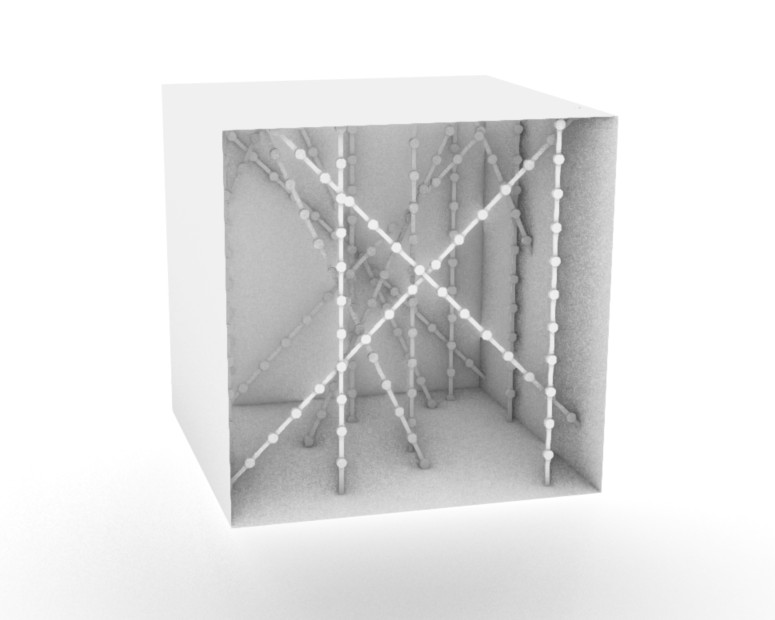
\includegraphics[width=0.7143\textwidth]{model.jpg}
    \caption{First Model of Box}
\end{figure}
\paragraph{}When designing the 1’x1’x1’ box frame, we wanted the space to be fully enclosed and allow for the “walls” to be interchangeable. These goals meant no light could come into the box and we could easily experiment with different materials to see how they interact with the LEDs. The box was 3D printed as six separate pieces as seen in Figure 2. Two for the top and base and four for the corner pieces. These six pieces joined together with a peg system at each corner. The 1’x1’’1/8” panels set into the base, slid into the corner pieces as seen in Figure 3, and were held in place by the top frame. Due to the nature of a 3D print, there were many iterations to make sure that everything fit into place perfectly. 
\begin{figure}
    \centering
    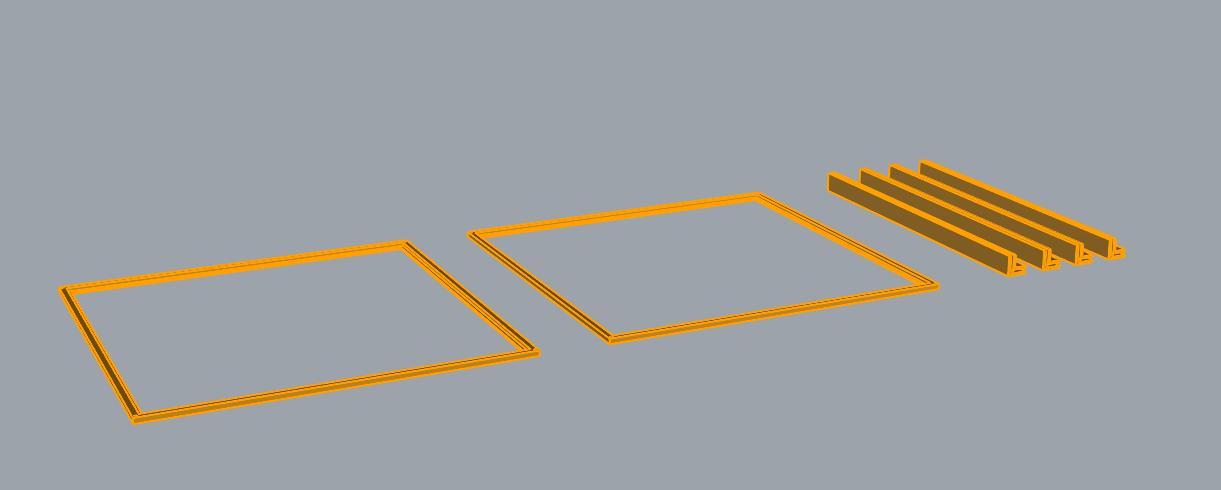
\includegraphics[width=0.7143\textwidth]{edges.png}
    \caption{3D Model of Side Pieces}
\end{figure}
\begin{figure}
    \centering
    
\includegraphics[width=0.7143\textwidth]{corner.png}
    \caption{3D Model of Edge Pieces}
\end{figure}

\paragraph{}Beginning to experiment with our box also led to some challenges. We came across the issue of materiality and did not have enough mirror panels to create a full mirror box like we had originally intended. As such, we experimented using dichroic panels and scrim as different side panels. Our first iteration of the box had 3 dichroic panels and a panel of scrim, as seen below in figure 4. The dichroic panels added vibrant, color shifting effects, and kept the reflective quality of the mirrors. The scrim was translucent and offered slight reflection and diffusion of light. However, during prototyping we decided that the scrim as one panel clashed with our original objectives . We ultimately decided to remove it from the design and fully dive into the dichroic panels.
\begin{figure}
    \centering
    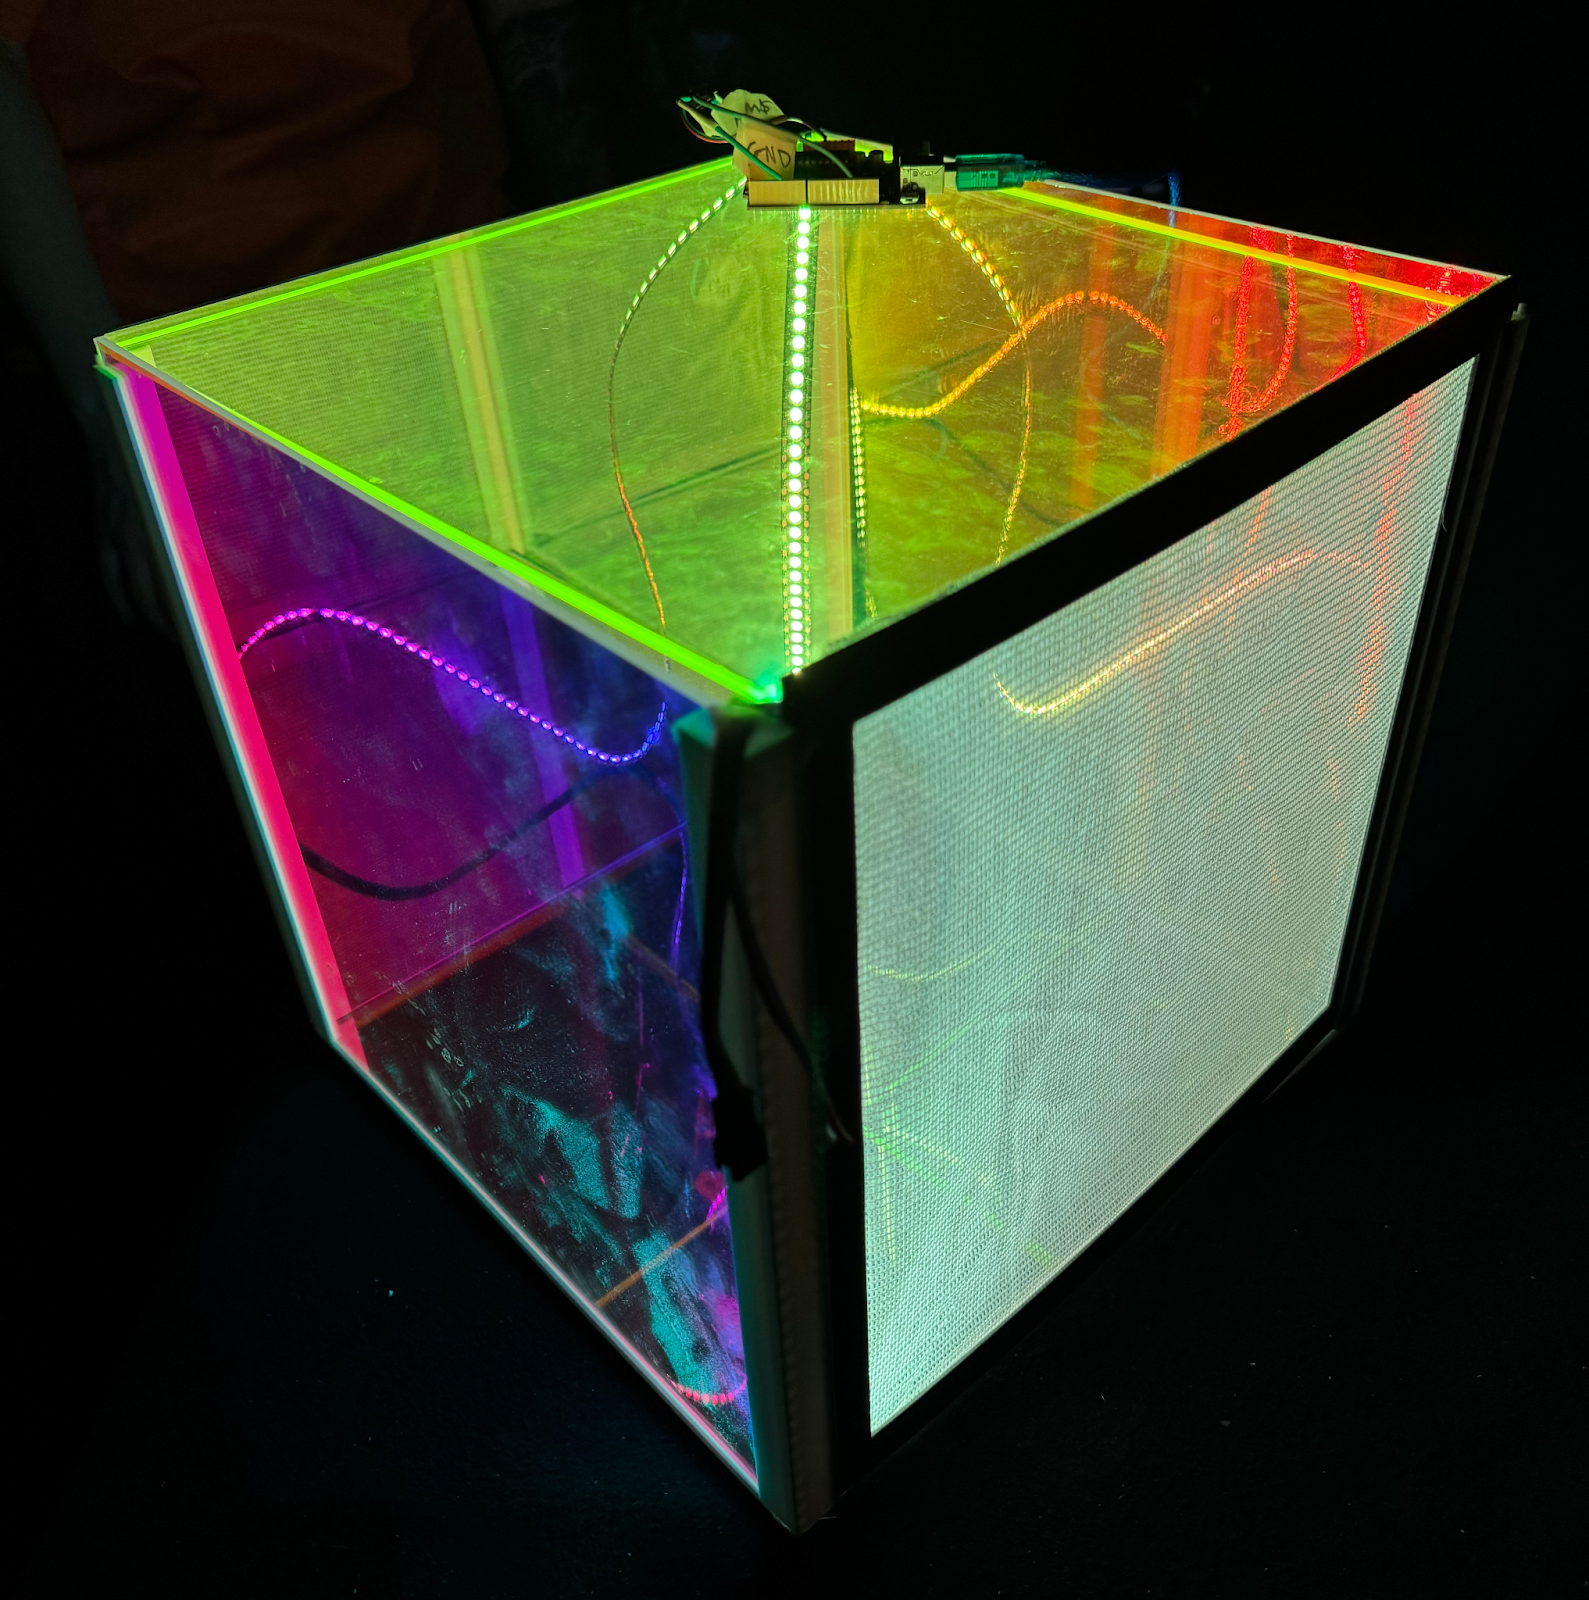
\includegraphics[width=0.7143\textwidth]{1st.png}
    \caption{First Iteration of Box}
\end{figure}


\paragraph{}From a technical standpoint, there was a lot to be explored with in terms of LEDs. First, we tried out multiple different colors and decided on using cool colors as cooler colors are often associated with space and science. They also created a better environment when placed in the box. Figure 5 shows some of the basic color options we first looked at. 
\begin{figure}
    \centering
    \rotatebox{270}{%
    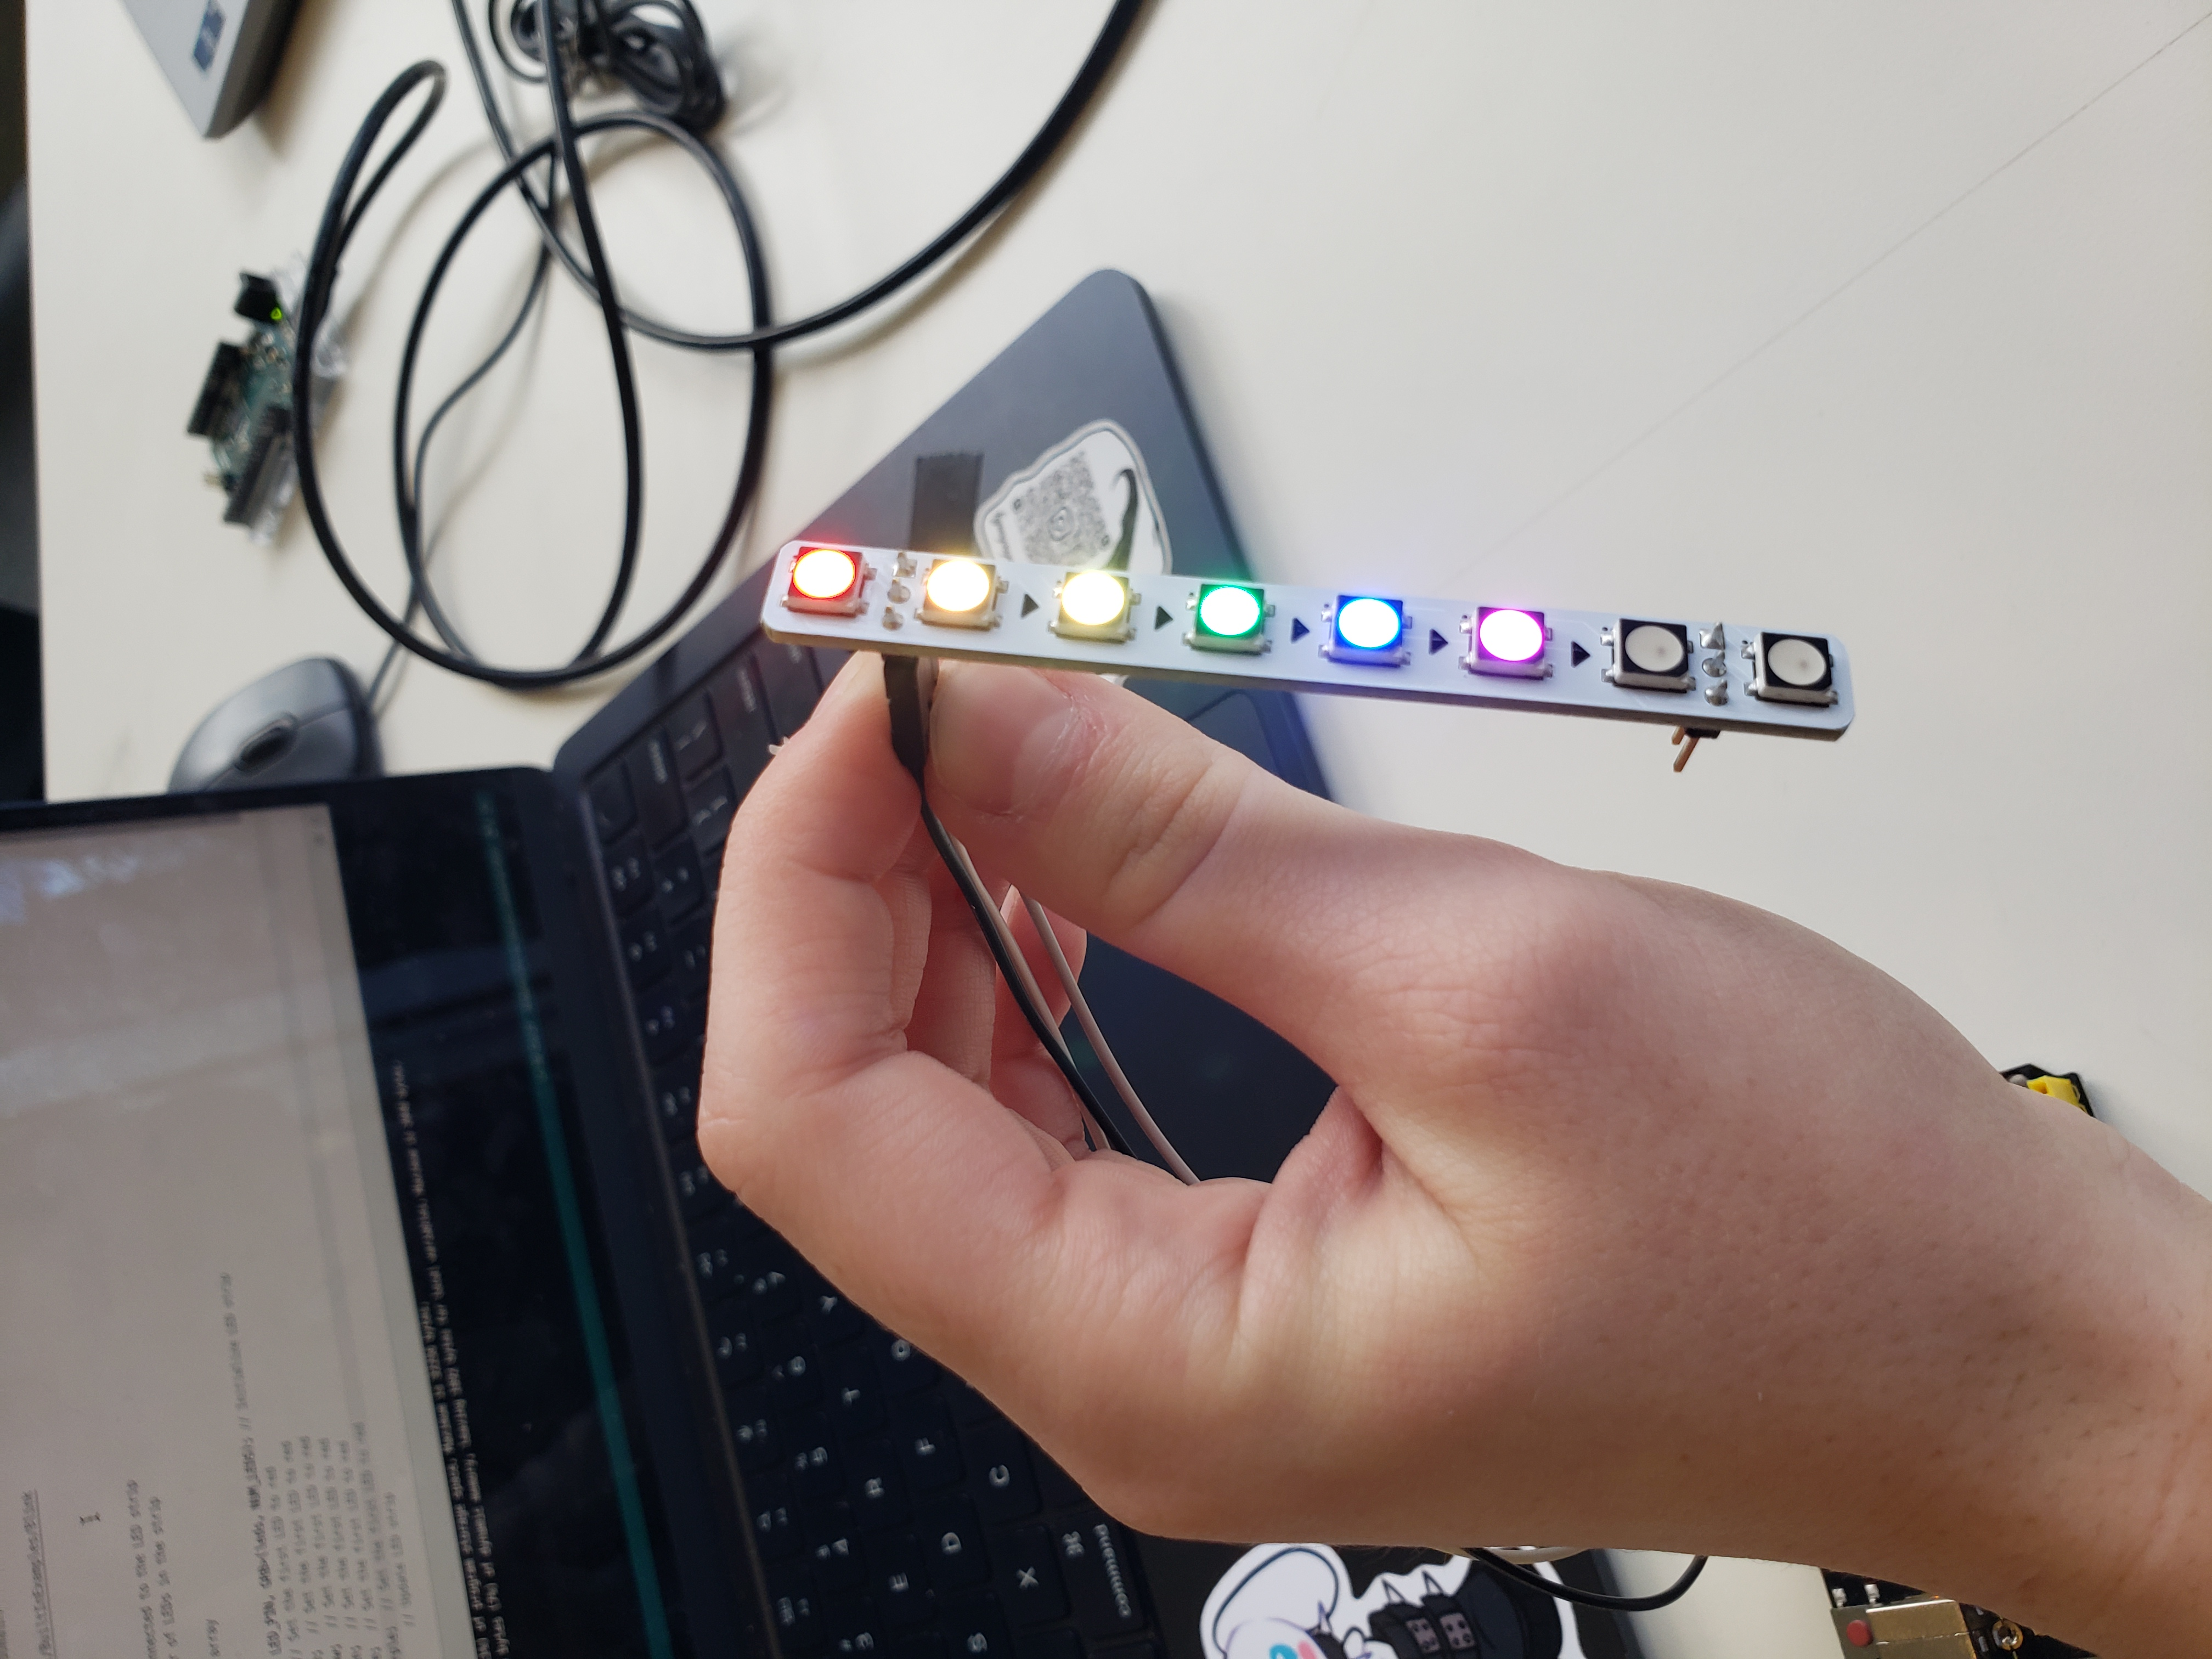
\includegraphics[width=0.7143\textwidth]{20250227_133329.jpg}}
    \caption{Basic LED Color Sample}
\end{figure}

\paragraph{}Our initial tests with LED strips exposed key challenges. Sending a basic signal to the LEDs created an unpleasant strobe effect, especially in a darkened space. This detracted from the intended smooth motion of the particles. This was made especailly obvious during the midterm review session. This in combination with outside advice we decided to animate the LEDs. This alleviated the strobe effect while also making it more obvious that the dot was supposed to be moving. 

\paragraph{}During this time we also struggled on how to display the LEDs from top to bottom and show different angles. After trial and error with the double sided tape on the LED strips, we came up with 3D printed “sticks” that would hold the strips in place and control the direction/path of the cosmic ray points. This can be seen in figure 6. The LEDs were then cut and attached to twelve sticks. These sticks fit into a 1’x1’x1” piece of wood that rested on top of our 3D box. Holes were drilled straight through at different angles so each strip was angled differently and the LEDs could be wired to the Arduino straight through the top. This created a brain above our projects as seen in figure 7. This did come with some drawbacks, though, as the Arduino could only power X many LEDs, this is to be expected, as parallel circuits often draw more power than circuits in series. 
\paragraph{}We also struggled with connection issues in terms of getting the LEDs to attach to our breadboard. We first tried to solder the pads on the LED strips to solid core wires then securing them with electrical tape. However this connection did not hold. This meant we had to look to other options. We then went to clips which would puncture the pads on the LEDs with one side and puncture the wires with the other. This worked and held well. However, they were difficult to remove and should be treated as permanent fixtures going forward. 

\paragraph{}When exploring the usages of the LEDs we tried to lean more into how they could be used to describe the different kinds of particles that we see as cosmic rays and how they can relate to a particle’s energy and distance traveled before decay. Thus, we made it so the distance that the animated dot would move was proportional to the intensity of the light that it would display. It was also related to the color that the LED would produce. This created an effect where after some time you could expect what a dot would do based on the color you first saw. 

\begin{figure}
    \centering
    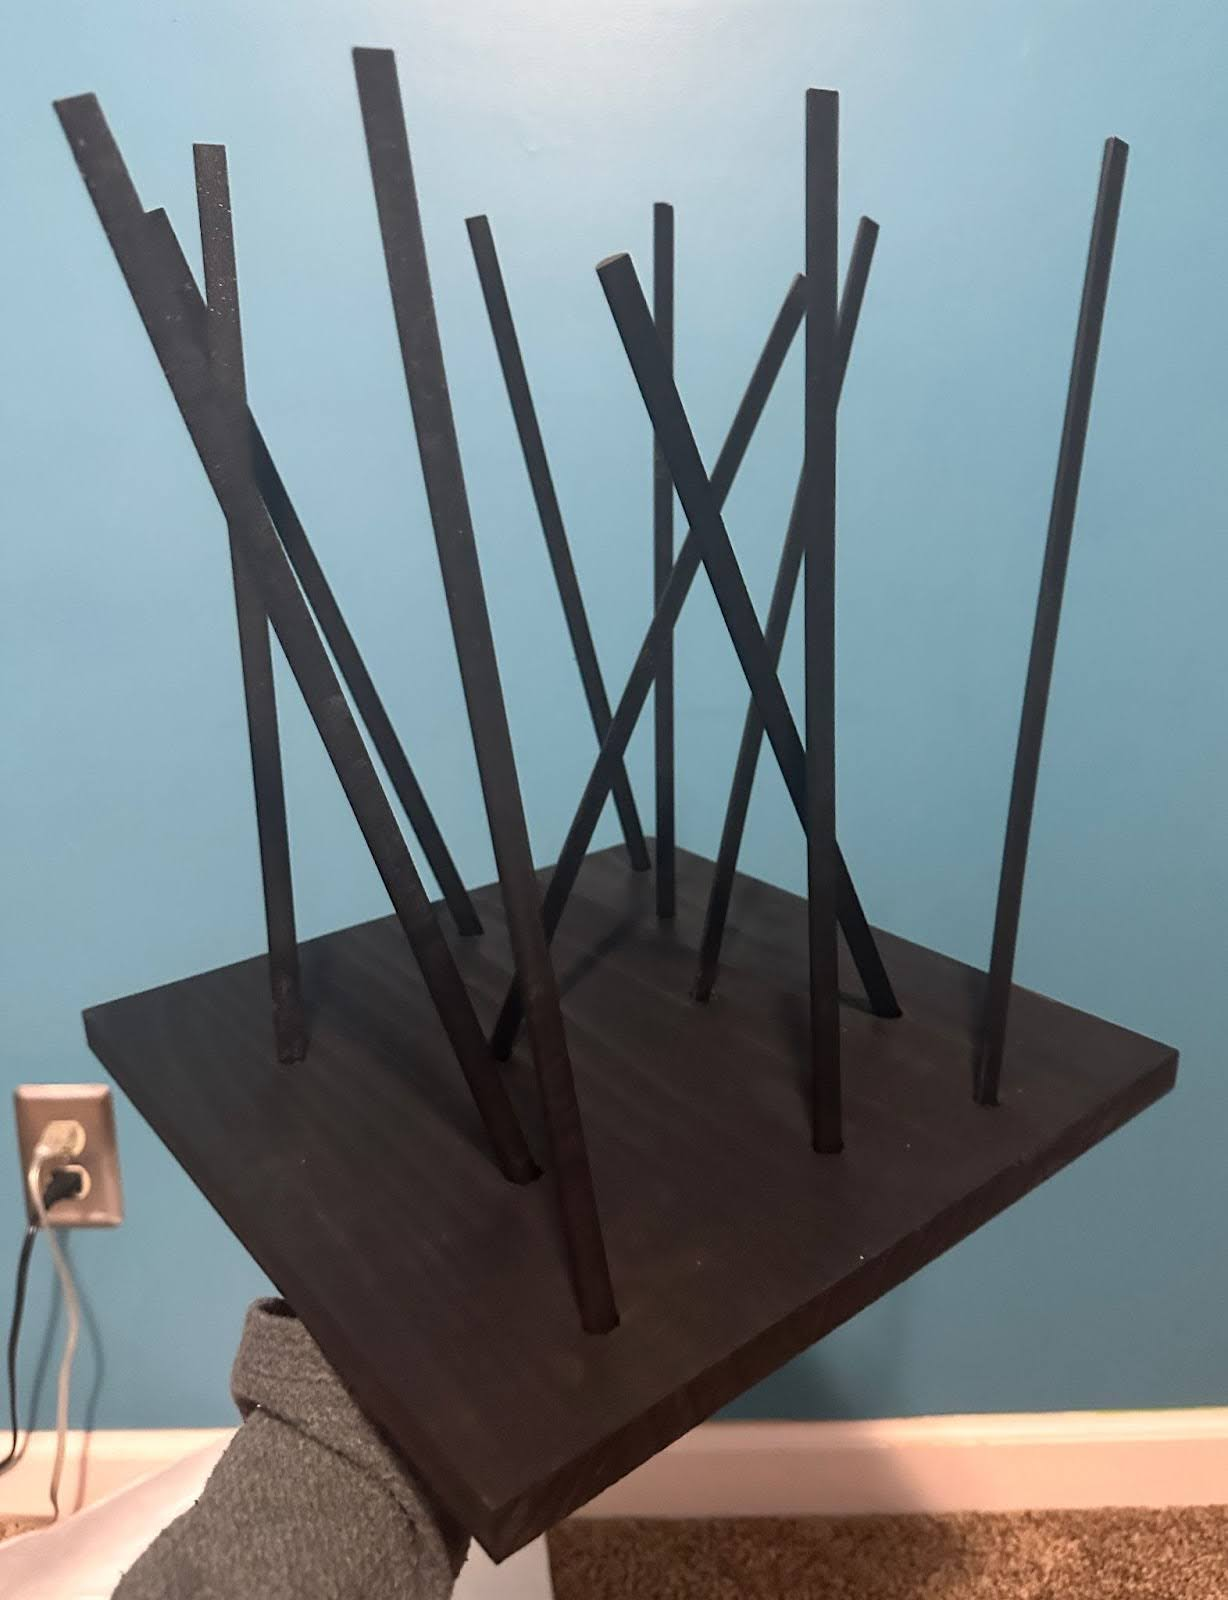
\includegraphics[width=0.7143\textwidth]{sticks.jpg}
    \caption{Roof Segment}
\end{figure}

\begin{figure}
    \centering
    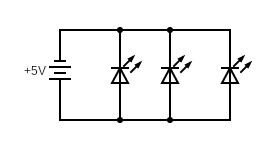
\includegraphics[width=0.7143\textwidth]{circuit.png}
    \caption{Simplified Schematic}
\end{figure}

\section{Outcomes}
\paragraph{}Figure 8 and 9 show the final outcome of the exhibit. A mirror and dichroic enclosure with multiple LED strands arranged in various angled paths. The variation in speed, brightness, and color are able to effectively communicate cosmic rays and their random behavior. The code for which can be found in the github:\href{https://github.com/EverettHagen/PHYS494}{here}

\begin{figure}
    \centering
    \rotatebox{270}{%
    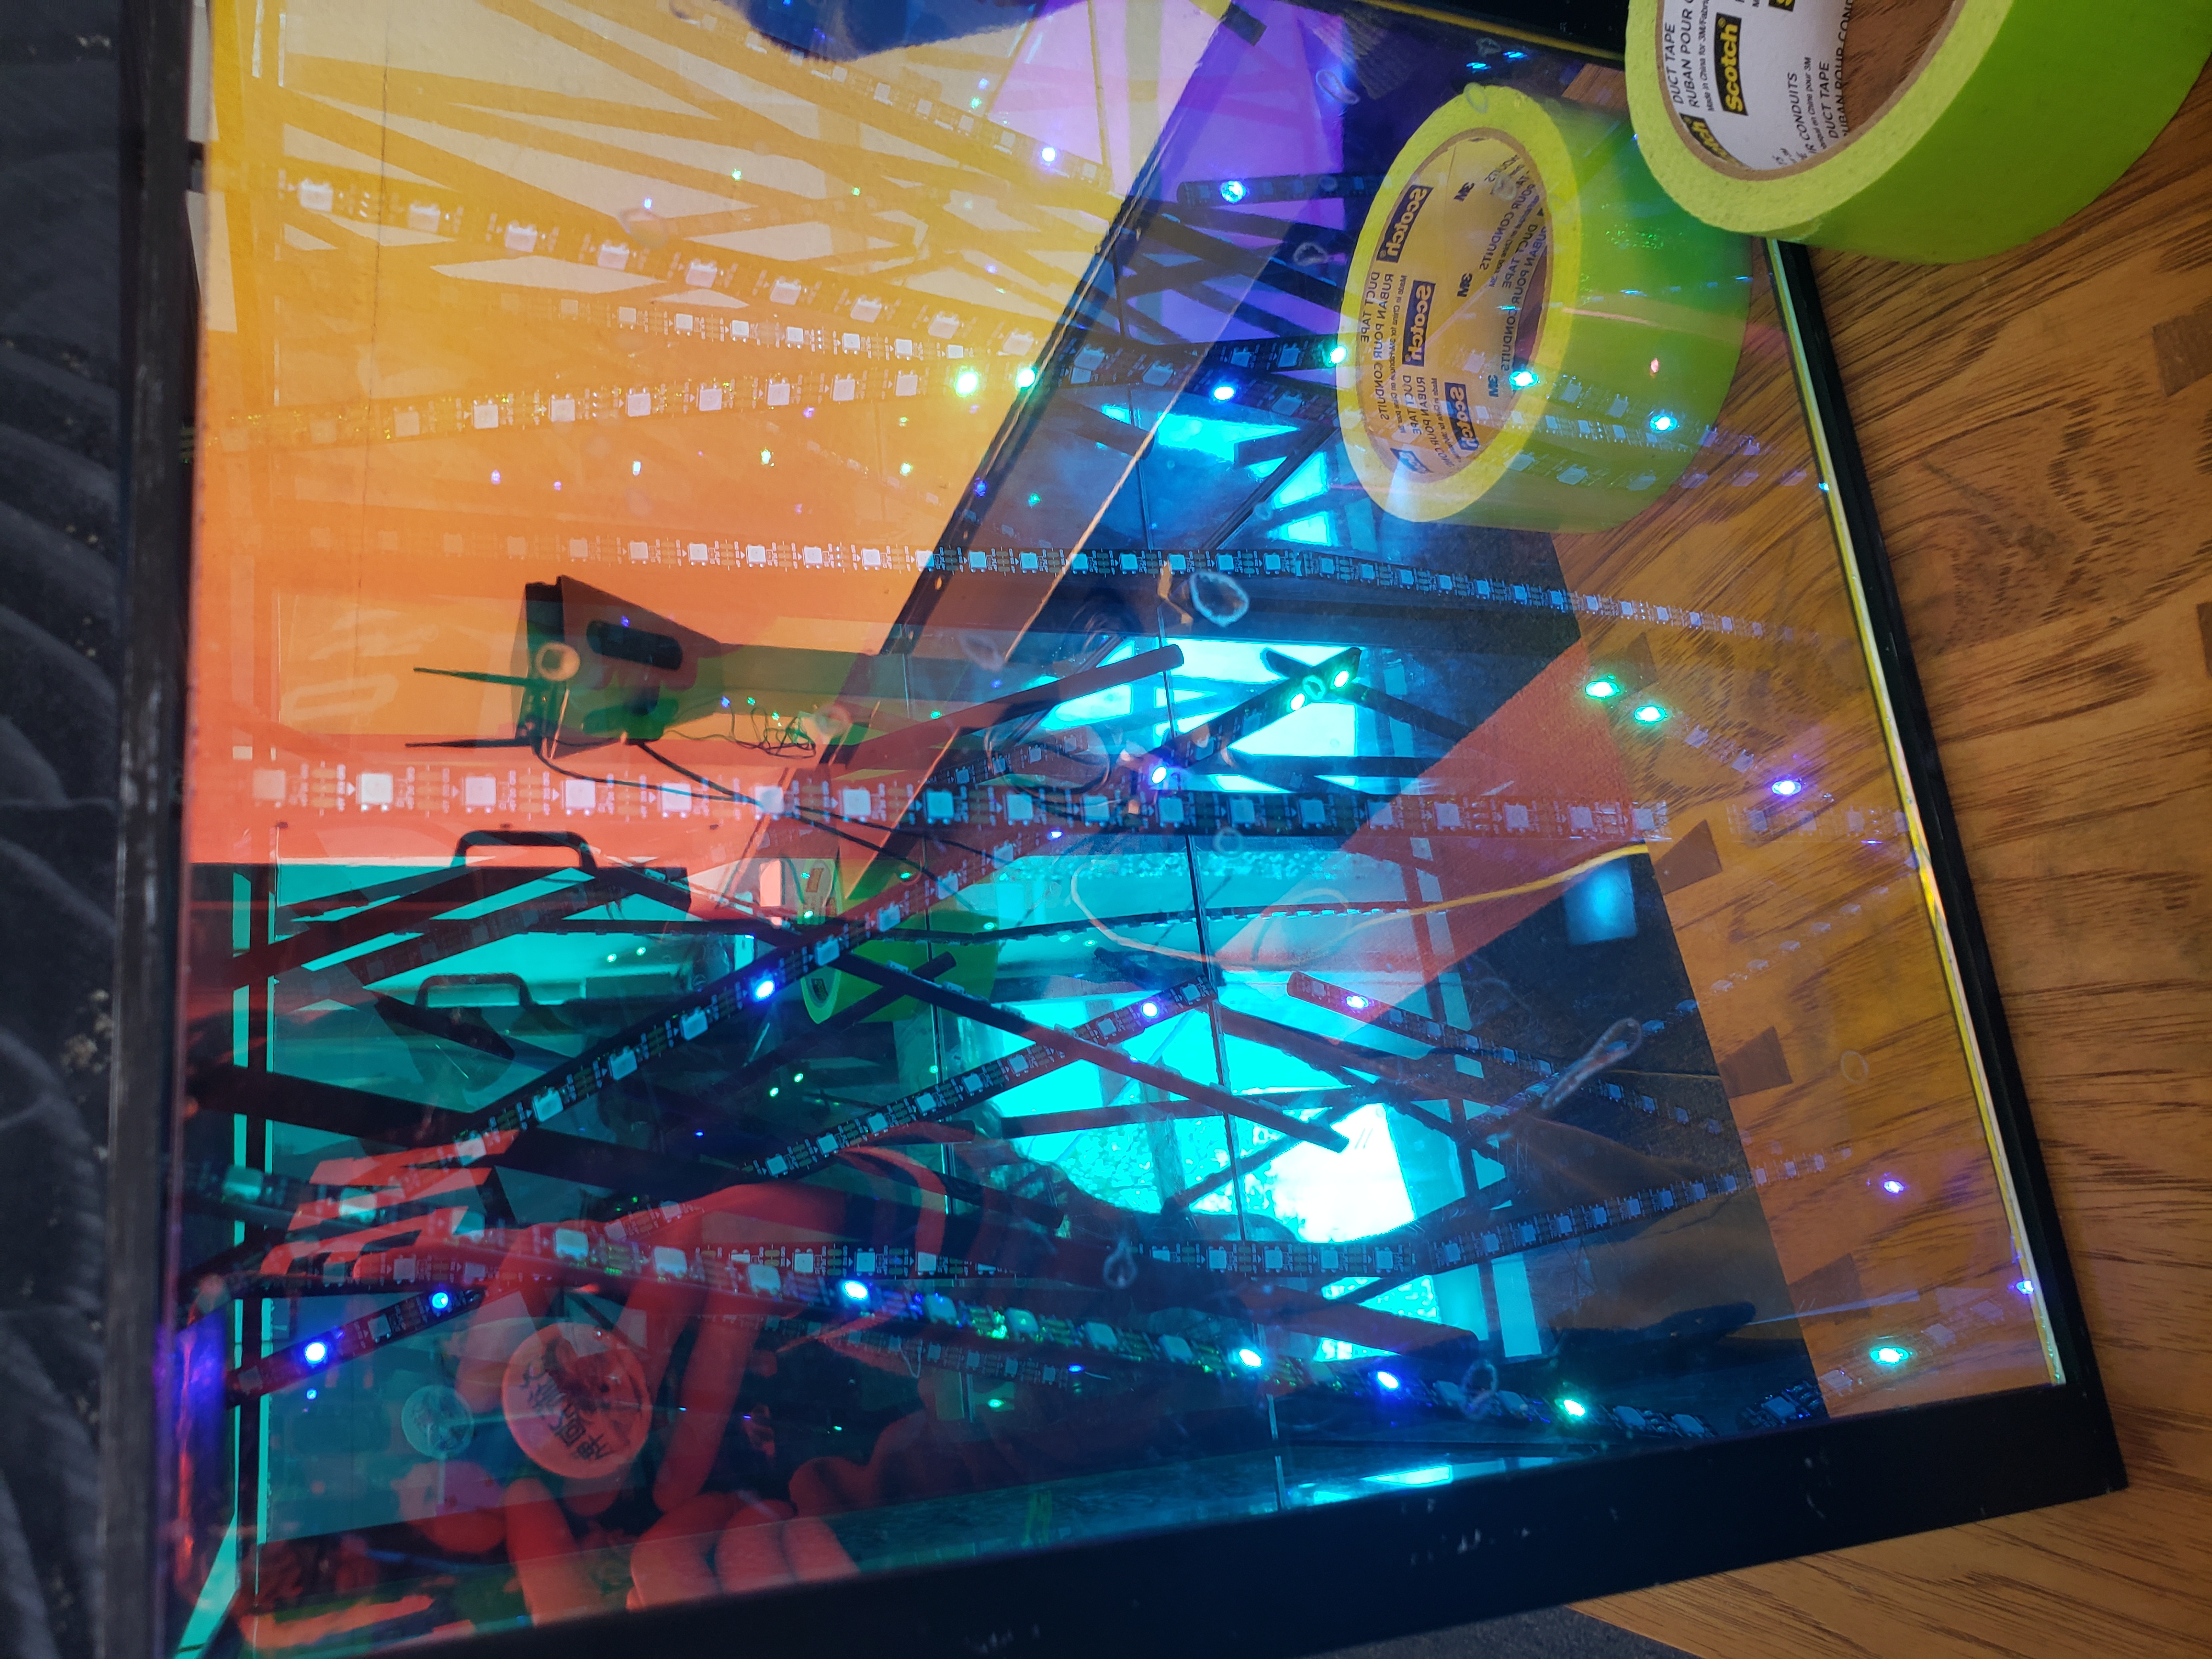
\includegraphics[width=0.7143\textwidth]{20250410_134826.jpg}}
    \caption{Final Status of Exhibit in Lit Room}
\end{figure}
\begin{figure}
    \centering
    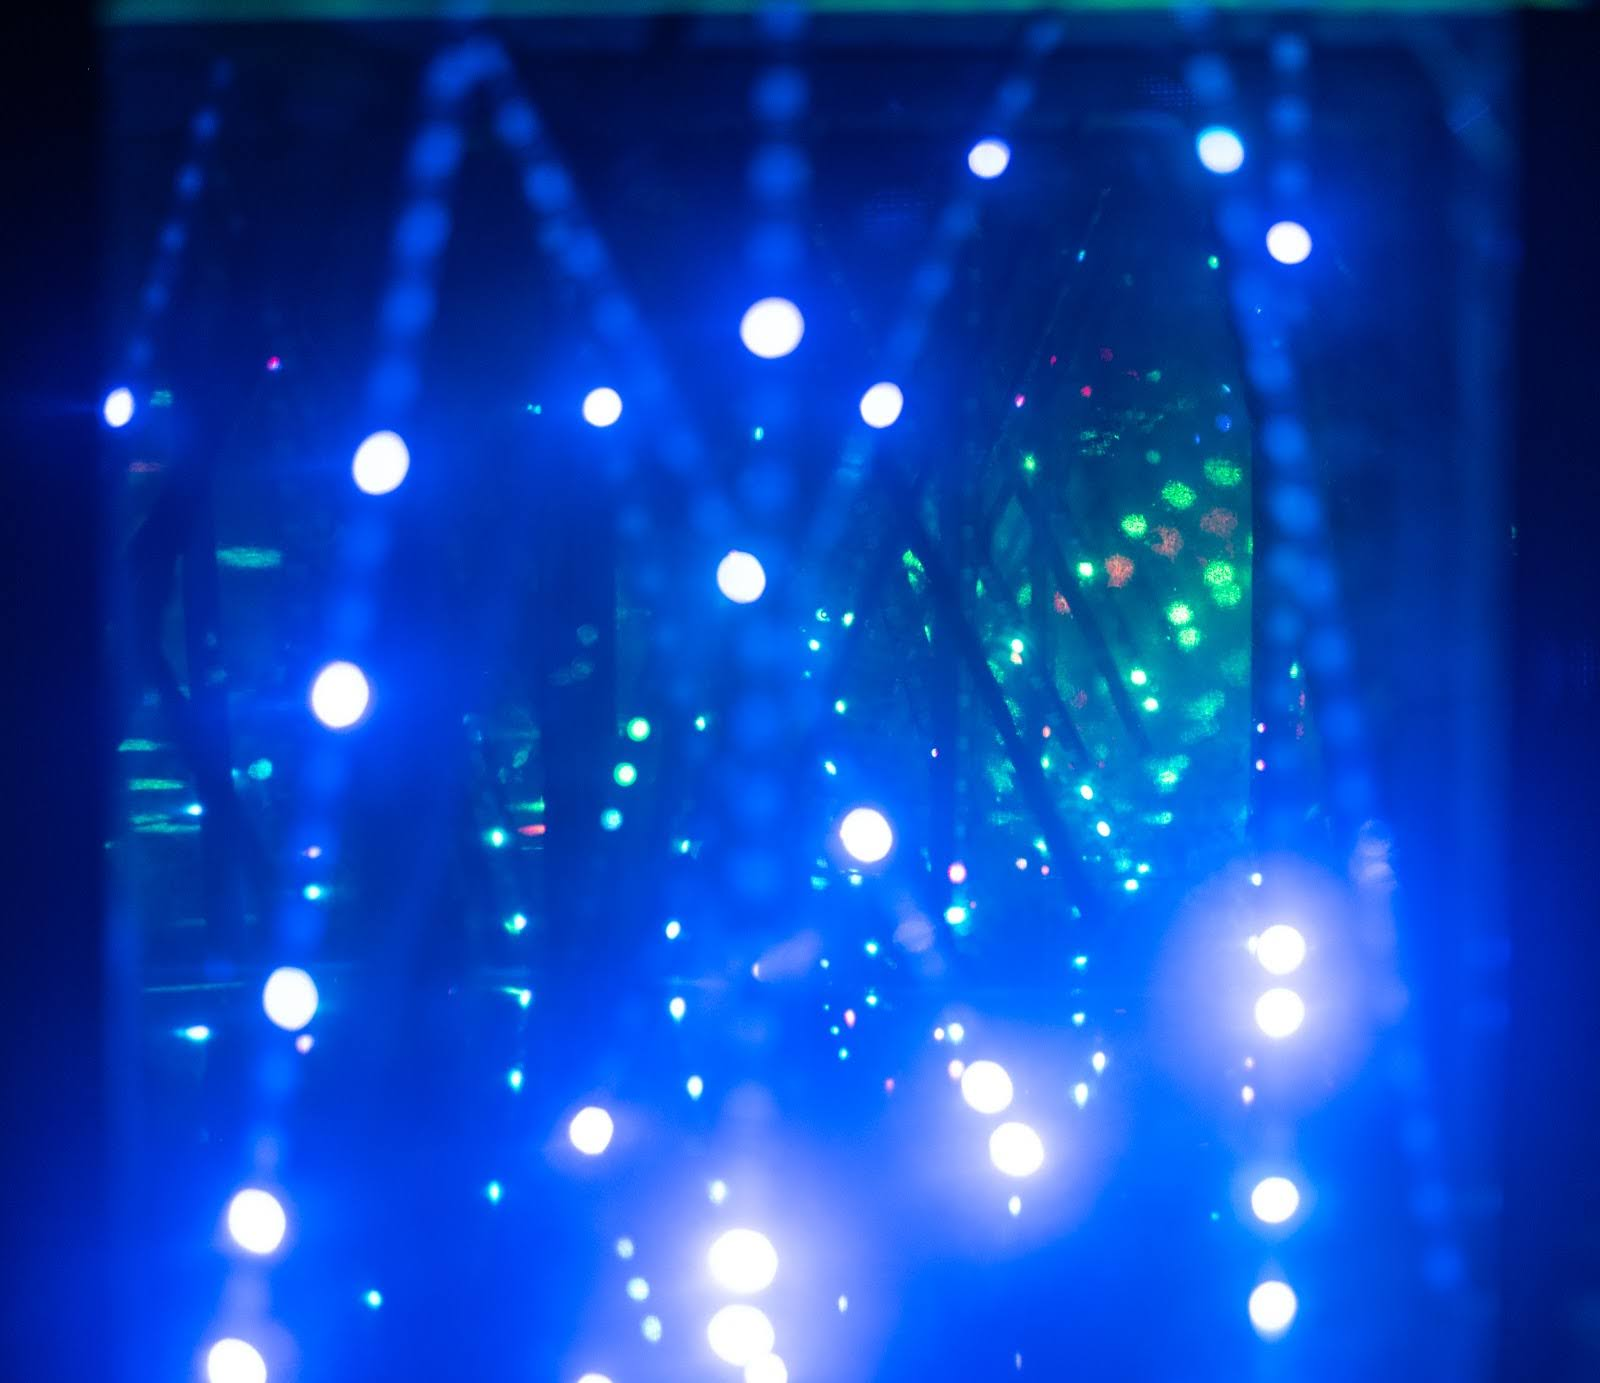
\includegraphics[width=0.7143\textwidth]{dark.jpg}
    \caption{Final Status of Exhibit in Dark Room}
\end{figure}

\paragraph{}To compliment our LED exhibit, we created a visual graphic that displays the life cycle of a cosmic ray. This graphic acts as a guide to form a basic understanding of a cosmic ray as well as their path of travel. Experiencing the LED exhibit evokes the awe of the cosmic rays, but might not fully communicate a total understanding without some initial information. This graphic helps develop a stronger understanding starting at the birth from a supernova to the interaction at Earth’s atmosphere. To appeal to younger children and people of all ages and backgrounds, we decided to personify the cosmic ray and create a character. This approach not only creates a better understanding, but is more engaging for the public, especially those who are not as interested or familiar with science.
\begin{figure}
    \centering
    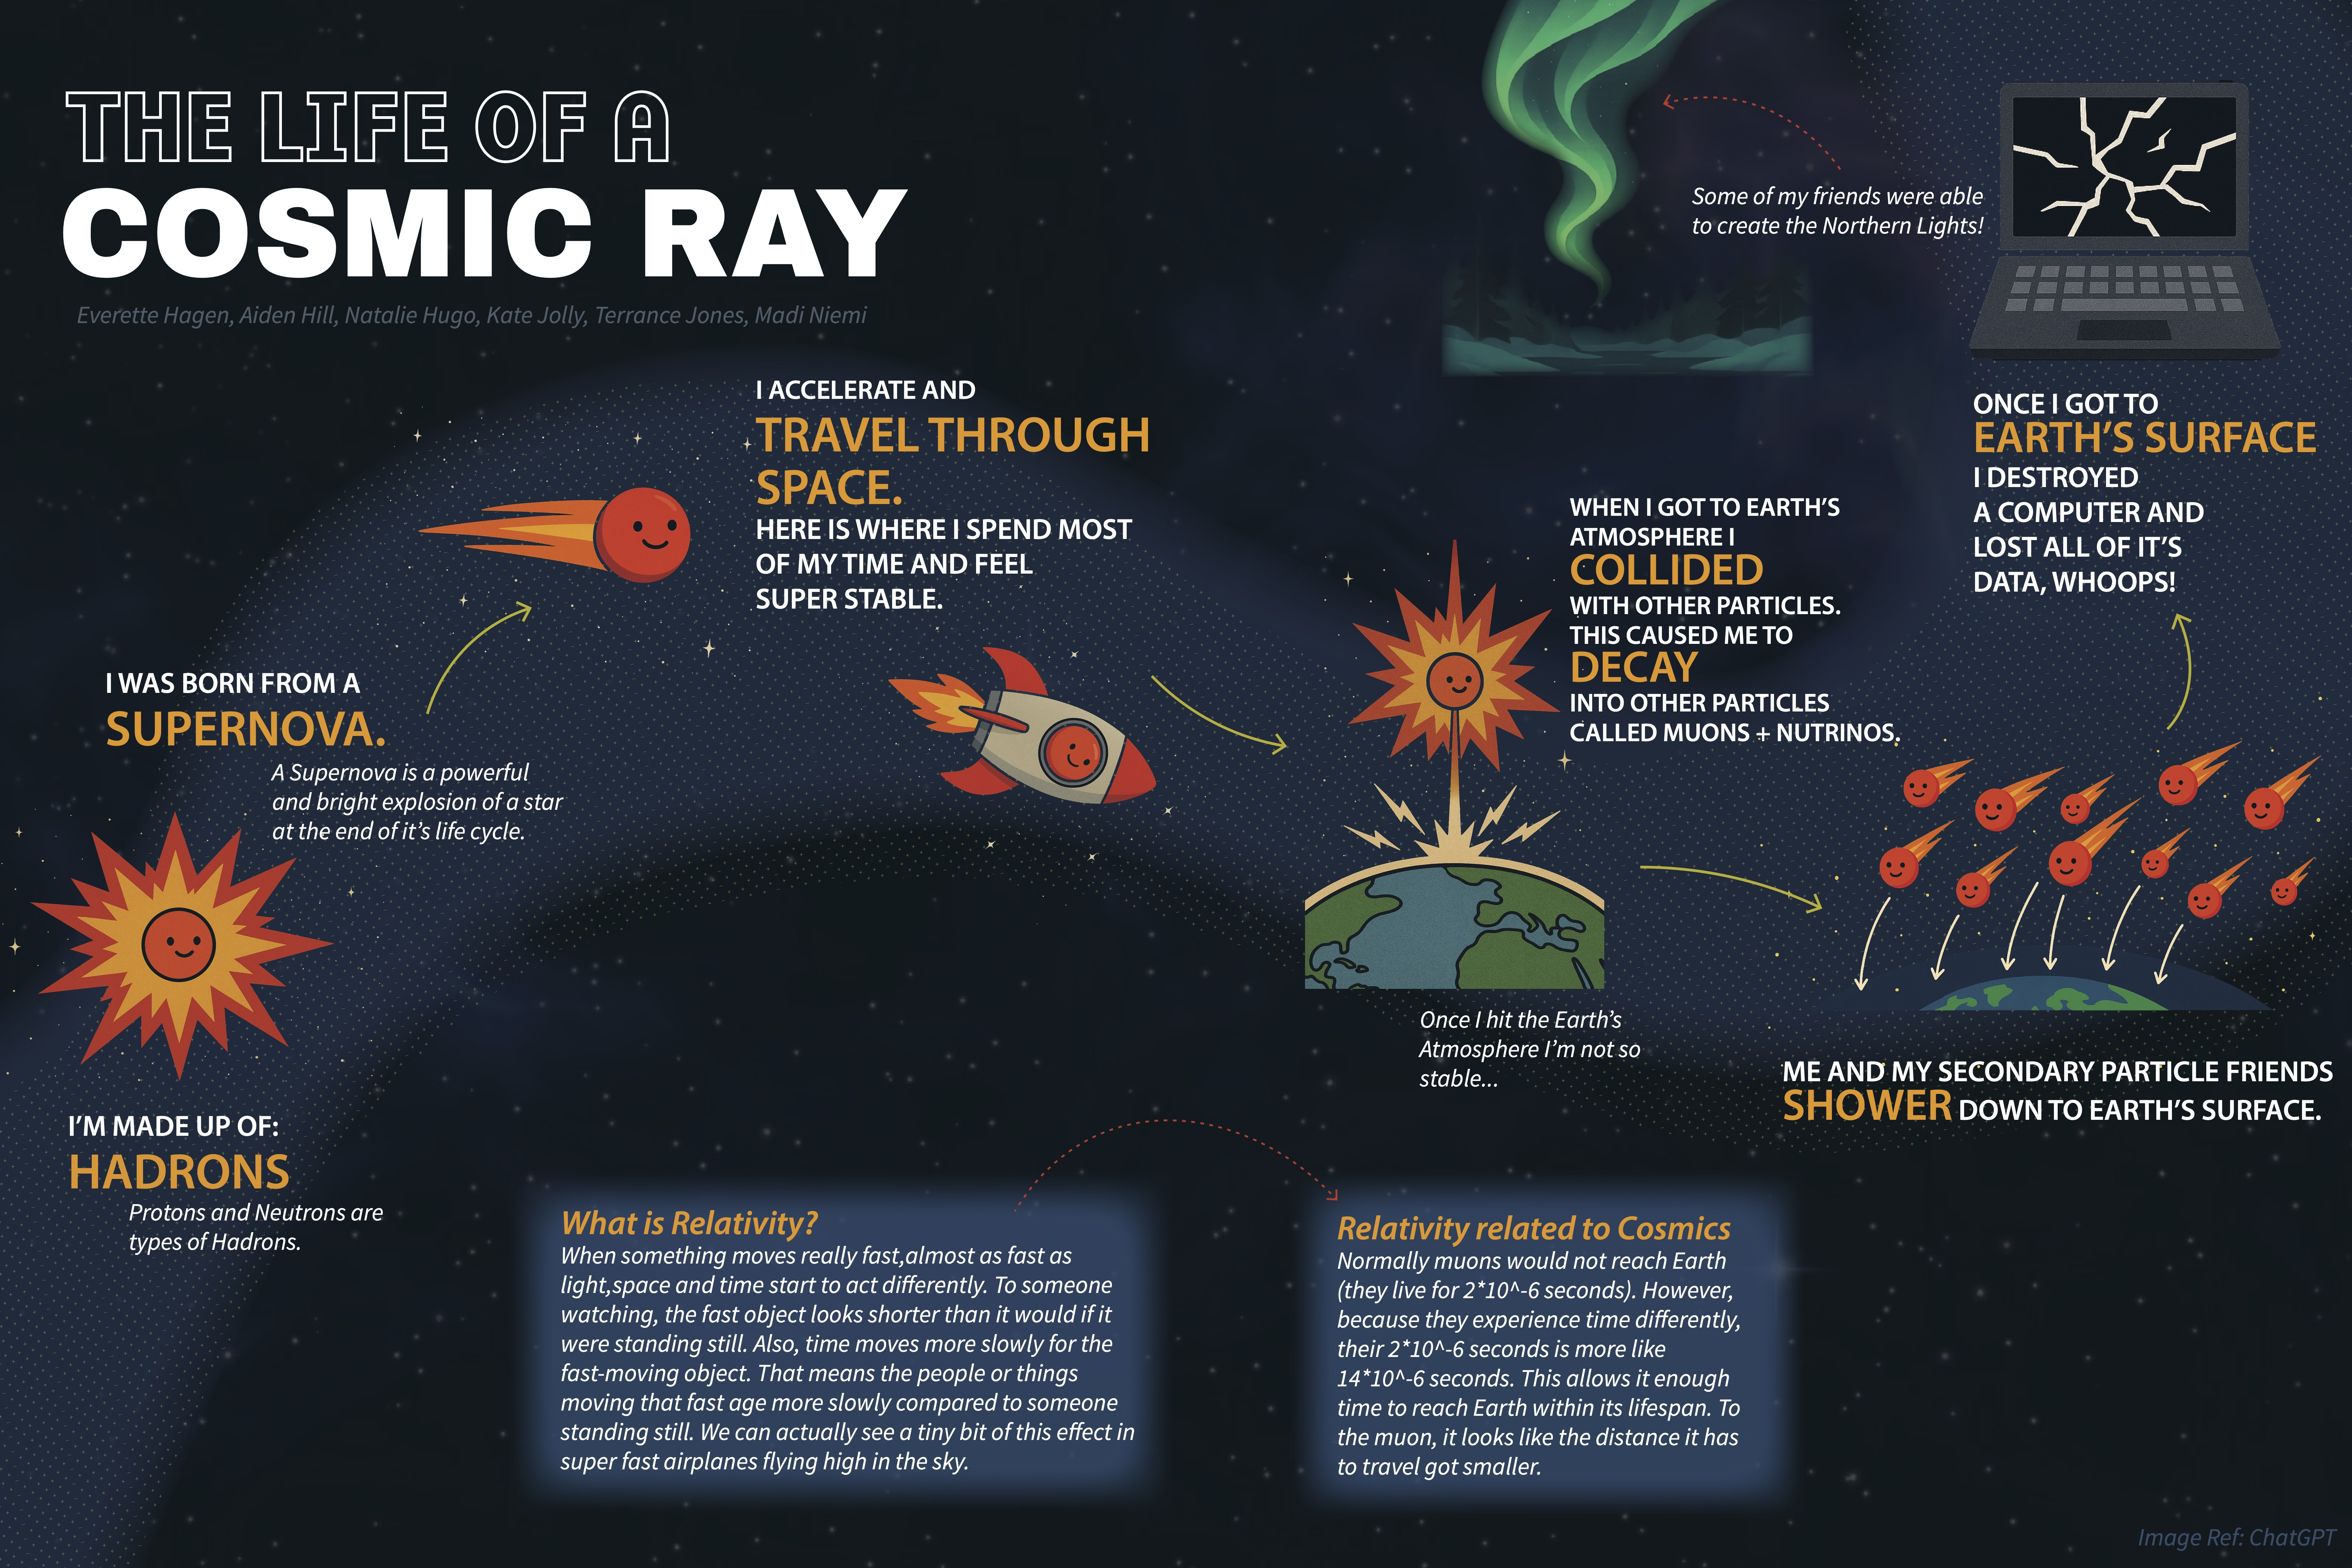
\includegraphics[width=0.7143\textwidth]{425-print.pdf}
    \caption{Visual Graphic of Cosmic Ray Life Cycle}
\end{figure}


\section{Critique of Outcomes}
\paragraph{}Some of the most essential things we found that related to our project was the simplicity of it. While it could be considered to have a lack of interesting components, it boils the essenic of what cosmic rays are down to their very core. It takes their complex ideas and turns them into something far more understandable. 
\paragraph{}Something that remained untested, but would be interesting to take into consideration is the introduction of another layer of LEDs which could mimic the air shower effect. So, having a layer where the singular LED strand would then split off into multiple more LED strips. We also think changing the way the LEDs fade off should be looked into. We were looking into the function fadeToBlackBy() as a way to implement the final LED to slowly turn off in order to represent decay. However, we were not able to get it working in time. We think this is something that should be further explored. 
\paragraph{}If we continue running with the idea that we currently have, we should leave out having varied textures as borders. When we tested it with scrim, we found that it didn’t add anything to the exhibit, but rather was just a bit of an eye sore. 
\paragraph{}Some of the feedback that we got on our final review really stuck with us. This included describing more about the true speed of cosmics. Also, having the LEDs be along the wall instead of all throughout the space so you can't physically see the strip. This truly embodies making the unseen, see

\section{Next Steps}
\paragraph{}We need to consider the feasibility of scaling a project similar to ours up. With our current project, there were already times when there was confusion as a result of how many wires we had. If we were to scale up, we would need to develop a better wiring organization system or find a system that requires fewer wires. We should also consider finding a setup in which our LEDs are organized in series rather than in parallel to avoid the power consumption issue that we came across during our process. There is an opportunity to include scintillators (cosmic ray detectors) to trigger specific LED paths as cosmics rays appear. This would increase both accuracy and user understanding.
\paragraph{}We would also like to consider ways to increase the viewer experience. This could be through exploring the addition of sounds that correspond to the ‘falling’ of the points. The easiest way we think this could be incorporated is to use instruments traditionally associated with the ‘falling’ motion. This could be through the usage of rain sticks, rain drums, or to create a more of a surreal experience something like a waterphone.
\paragraph{}Another implementation that we would have liked, however due to resources were not able to fulfill is the usage of thinner standalone LED strands. Something more akin to fairy lights. This would make the exhibit feel less stagnant as the LEDs would have a free range of motion. This could also make the experience more interactive as viewers could move the strands. 

\section{Conclusion}
\paragraph{}Through our experimentation in representing cosmic rays as points, we created a compelling model that explains cosmic phenomena through an immersive experience. The dichroic panels and animated LEDs provided a visually engaging display that reflected the randomness of cosmic rays, sparking curiosity and encouraging viewers to learn more about the phenomenon. Our experiments with materials, color, and coding allowed us to test various visualization and representation techniques, helping us refine our model to emphasize the most important aspects. Ultimately, our model achieved its goal of invoking awe and laid the groundwork for future iterations.
\paragraph{}We hope those who follow in our footsteps can advance what we started. May the foundation we created allow you to dive deeper than we were able to. We invite you to come to find your own sense of meaning to this project and explore new possibilities. 
\end{document}
